% !TeX spellcheck = it_IT
% !TEX TS-program = pdflatex
% !TEX root = ../main.tex


% ********************************************************************
\section{Prototipo}
\label{sec:prototipo}
% ********************************************************************


\subsection{Login e autenticazione}

La procedura di \textit{login} avviene esclusivamente attraverso l'interfacciamento con \textit{Metamask}, che funge da interfaccia tra l'utente e la rete \textit{blockchain}.



\subsection{Dashboard donatore}
La \textit{dashboard} del donatore è l'interfaccia attraverso la quale gli utenti possono interagire direttamente con la piattaforma a seguito della procedura di autenticazione. \\ Essa è progettata per fornire una visione sintetica e intuitiva delle iniziative di \gls{cf} attive, permettendo all'utente di monitorarne lo stato di avanzamento (ad esempio, attraverso il \textit{budget} raggiunto e la scadenza). \\
Una volta selezionata l’iniziativa di interesse, l’utente ha la possibilità di procedere con l’operazione di donazione. In particolare, il sistema adotta il meccanismo di raccolta \textit{keep-it-all}, in base al quale l’Ente beneficiario conserva i fondi raccolti anche qualora l’obiettivo economico prefissato non venga raggiunto entro i termini prestabiliti.
Tale scelta progettuale risulta coerente con la categoria di Enti autorizzati alla creazione delle iniziative sulla piattaforma, individuati esclusivamente negli Enti del Terzo Settore, per i quali anche contributi parziali possono risultare funzionali al perseguimento delle finalità sociali.


\begin{figure}[!h]
	\centering
	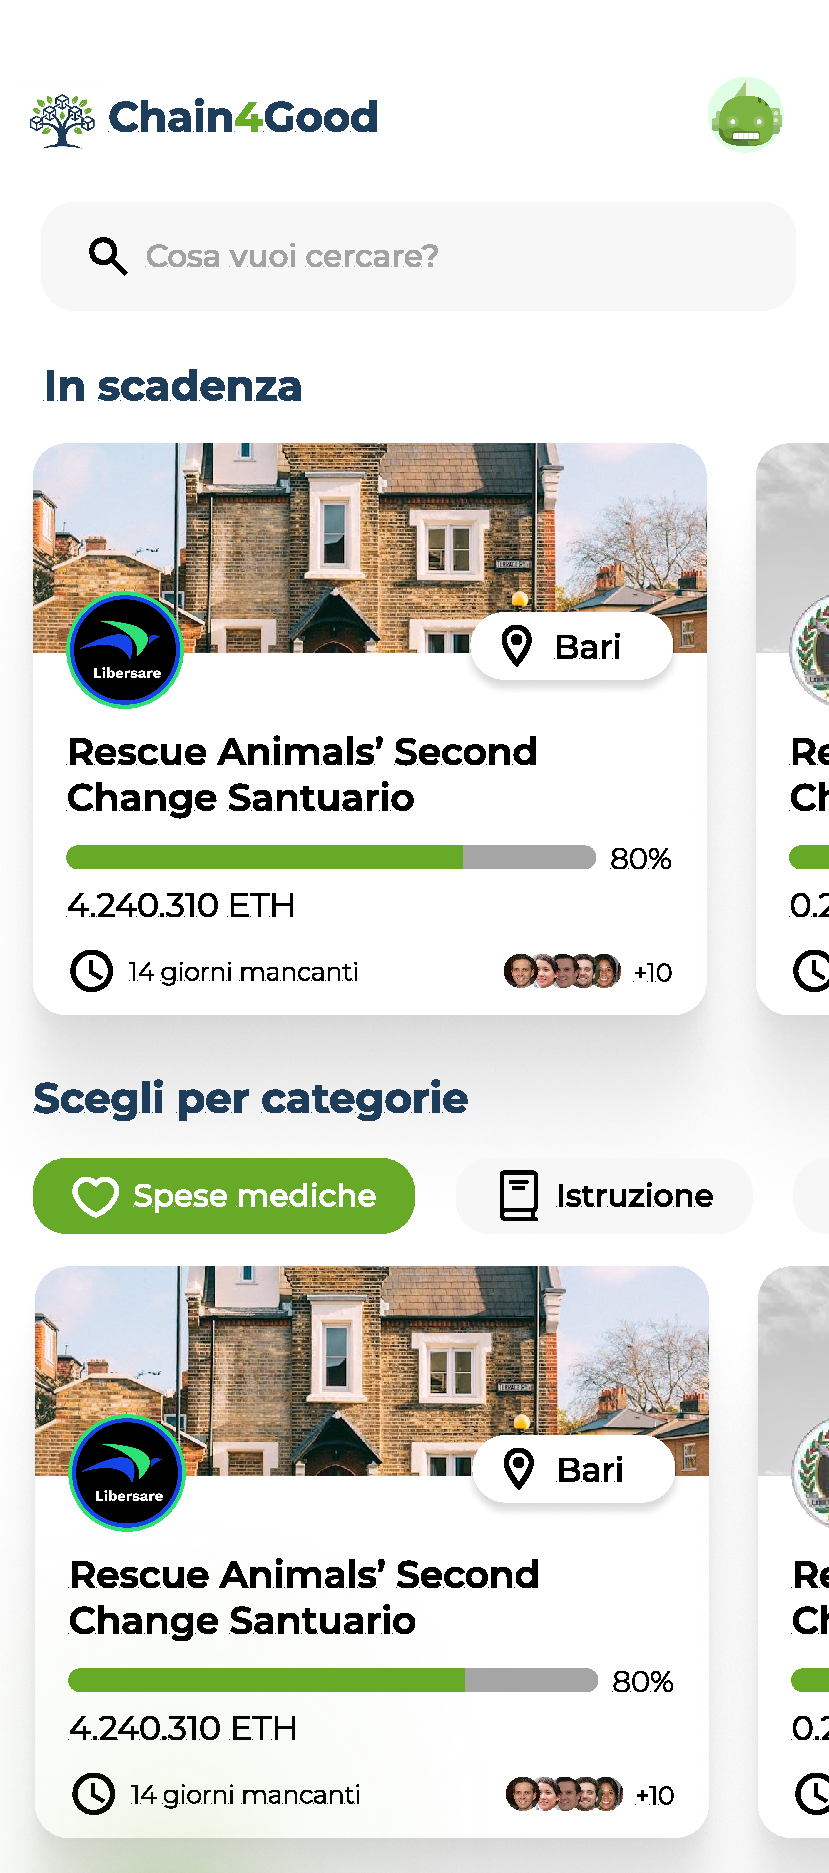
\includegraphics[width=0.37\textwidth]{images/Home_nuova.pdf}
	\caption{Dashboard del donatore}
	\label{fig:dashboard-donatore}
 \end{figure}

\subsection{Creazione progetto}
	La creazione di un progetto costituisce l’atto attraverso il quale il beneficiario formalizza la propria proposta sulla piattaforma. Tale procedura si articola in due step (\ref{fig:inserimento progetto}):

\begin{itemize}
	
	\item Step 1: l'Ente è tenuto a specificare le informazioni fondamentali del progetto, quali il nome, la categoria di appartenenza, l’obiettivo economico e il termine temporale della raccolta fondi. \\ 
	Gli ultimi due parametri permettono di automatizzare la gestione delle risorse in modalità \textit{trustless}, in quanto vengono utilizzati dallo \textit{Smart Contract} per determinare l’esito della campagna di \gls{cf};
	
	\item Step 2: prevede l’inserimento di un piano dettagliato delle spese, oltre ad una descrizione approfondita del progetto e un’immagine di copertina. Tale prospetto non assolve solo finalità informative, ma contribuisce ad incrementare la credibilità dell'iniziativa e a consolidare il rapporto di fiducia con i donatori. 
	
\end{itemize}


\begin{figure}[!h]
	\centering
	\begin{minipage}{0.37\textwidth}
		\centering
		\includegraphics[width=\textwidth]{images/nuovo_progetto1.pdf}
	\end{minipage}
	\hspace{1.5cm}
	\begin{minipage}{0.37\textwidth}
		\centering
		\includegraphics[width=\textwidth]{images/NuovoProgetto 2.pdf}
	\end{minipage}
	\caption{Inserimento di un nuovo progetto}
	\label{fig:inserimento progetto}
\end{figure}



\subsection{Inserimento e valutazione spesa}
A differenza dei sistemi centralizzati in cui l'Ente ha piena e immediata disponibilità del \textit{budget} donato, l’architettura proposta prevede che i fondi raccolti rimangano vincolati all'interno di uno \textit{Smart Contract}. \\
Per poter accedere a tali risorse, il beneficiario deve formalizzare una "Richiesta di Spesa" (\ref{fig:valutazione-spesa}) attraverso l'inserimento dei seguenti parametri: nome della spesa, importo richiesto, finalità dell'esborso e preventivo. \\
La sottomissione di una nuova richiesta di spesa, tuttavia, è vincolata al caricamento della prova di acquisto relativa alla richiesta precedentemente approvata dalla comunità di votanti (insieme degli individui che finanzia un'iniziativa di \gls{cf}).
Tale approccio serve per garantire un utilizzo progressivo e verificabile dei fondi raccolti, e ad assicurare la conformità delle spese per le finalità dichiarate.

\begin{figure} [h]
	\centering
	\begin{minipage}{0.37\textwidth}
		\centering
		\includegraphics[width=\textwidth]{images/nuova_spesa.pdf}
	\end{minipage}
	\hspace{1.5cm}
	\begin{minipage}{0.37\textwidth}
		\centering
		\includegraphics[width=\textwidth]{images/valutazione_spesa.pdf}
	\end{minipage}
	\caption{Valutazione di una richiesta di spesa}
	\label{fig:valutazione-spesa}
\end{figure}



\subsubsection{Meccanismo di validazione}
Per evitare lo stallo decisionale, lo \textit{Smart Contract} è stato programmato per agire secondo le seguenti regole:
\begin{itemize}
	\item La richiesta è approvata se la maggioranza dei votanti esprime un parere favorevole. In presenza di una partecipazione parziale, la soglia di maggioranza viene ricalcolata in funzione dei soli voti espressi.
	\item Qualora non venga registrata alcuna attività di voto, invece, il sistema approva automaticamente la richiesta.
\end{itemize}

Al soddisfacimento dei requisiti di approvazione, lo \textit{Smart Contract} esegue in modo autonomo e irreversibile il trasferimento della somma raccolta verso il \textit{wallet} del beneficiario. 


